\section{NLP and Computational Lexical Resource Techniques}\label{nlp}
Natural language processing (NLP) is a computational method for the automated analysis and representation of human language \cite{cambria2014jumping}. NLP techniques offer potential advantages to improve the quality of USs and can be used to parse, extract, or analyze user story's data. It has been widely used to help in the software engineering domain (\emph{e.g.}, managing software requirements \cite{Arias2018}, extraction of actors and actions in requirement document \cite{al2018use}.

NLP techniques are usually used for text preprocessing (\emph{e.g.}, tokenization, \emph{Part-of-Speech} (POS) tagging, and dependency parsing). Several NLP approaches can be used (\emph{e.g.}, syntactic representation of text and computational models based on semantic features). Syntactic methods focus on word-level approaches, while the semantic focus on multiword expressions \cite{cambria2014jumping}.

A computational lexicon resource is a systematically organized repository of words or terms, complete with linguistic and semantic data. These lexicons play a pivotal role in facilitating NLP systems focused on semantic analysis by offering comprehensive insights into language elements, encompassing word forms, part-of-speech (POS) categories, phonetic details, syntactic properties, semantic attributes, and frequency statistics. Lexical classes, defined in terms of shared meaning components and similar (morpho-) syntactic behavior of words, have attracted considerable interest in NLP \cite{cambria2014jumping}. These classes are useful for their ability to capture generalizations about a range of (cross-) linguistic properties. NLP systems can benefit from lexical classes in a number of ways. As the classes can capture higher level abstractions (\emph{e.g.} syntactic or semantic features) they can be used as a principled means to abstract away from individual words when required. Their predictive power can help compensate for lack of sufficient data fully exemplifying the behavior of relevant words \cite{kipper2006extending}.

Upon the completion of the transformation of USs utilizing a Conditional Random Fields (CRF) approach, wherein entities, actions (both primary and secondary), persona, and their relational attributes (specifically, triggers, targets and contains) are meticulously annotated and structured as a graph-based representation, a preliminary imperative emerges. This imperative entails the determination of a representative semantic interpretation for the ascertained actions. This determination, in turn, serves as a prerequisite for the generation of corresponding transformation rules, namely, \enquote{create}, \enquote{delete} and \enquote{forbidden} rules.

The attainment of this representative semantic interpretation hinges upon the application of a suite of foundational lexical resource techniques of a conceptual nature. These techniques assume a pivotal role in furnishing the essential cognitive infrastructure, facilitating a comprehensive grasp of the semantic roles, syntactic characteristics, and the systematic categorization to \enquote{creation}, \enquote{deletion} and \enquote{forbiddance} of linguistic elements embedded within the construct of the US.

Next, we will undertake a systematic examination of various computational lexical resource techniques. Subsequently, we will conduct a comparative analysis to determine the optimal approach for integration into our approach. 
\subsection{WordNet} \label{wordnet}
WordNet is an online lexical database designed for use under program control. English nouns, verbs,
adjectives, and adverbs are organized into sets of synonyms, each representing a lexicalized concept. Semantic relations link the synonym sets \cite{miller1990introduction}. 

WordNet operates by classifying words into four core syntactic categories: nouns, verbs, adjectives, and adverbs, collectively referred to as open-class words (see Table \ref{tb:wordnet}). This categorization allows for versatile language analysis and interpretation. For instance, words like "back," "right," or "well" can be interpreted differently based on their linguistic context, and thus, WordNet separately incorporates these varied interpretations \cite{miller1995wordnet}.

WordNet not only addresses word forms but also considers their inflectional morphology, accommodating the linguistic nuances that can arise due to different syntactic categories. For instance, when information is sought for \enquote{went}, the system intelligently provides relevant details about the verb \enquote{go}. On the other hand, derivational and compound morphology, encompassing words like \enquote{interpret}, \enquote{interpreter}, \enquote{misinterpret}, and so forth, are acknowledged as distinct entities within WordNet, despite sharing a common root.

One of WordNet's key strengths lies in its incorporation of various semantic relations, meticulously chosen to serve the broader scope of the English language. These relations are designed to be user-friendly and intuitively understandable, making them accessible even to individuals without advanced linguistic training. WordNet's semantic relations encompass \cite{miller1995wordnet}:
\begin{itemize}
\item Synonymy: The fundamental relation in WordNet, which employs sets of synonyms (synsets) to encapsulate word senses. This relation is symmetric and connects different word forms that share the same sense.
\item Antonymy (opposing-name): A symmetric relation that highlights opposing word forms, particularly vital in organizing the meanings of adjectives and adverbs.
\item Hyponymy (sub-name) and Hypernymy (super-name): These transitive relations between synsets organize noun meanings into hierarchical structures, with hypernyms representing broader categories and hyponyms representing specific instances or subcategories.
\item Meronymy (part-name) and Holonymy (whole-name): These complex relations delineate the component parts, substantive parts, and member parts of various concepts within WordNet.
\item Troponymy (manner-name): Similar to hyponymy but applicable to verbs, troponymy results in hierarchies that are typically shallower.
\item Entailment Relations: WordNet also accounts for entailment relations between verbs, capturing the logical inferences that can be drawn from certain actions.
\end{itemize}
These semantic relations are represented in WordNet through pointers, establishing connections between word forms and synsets. In total, WordNet incorporates more than 116,000 of these pointers, facilitating the exploration of intricate semantic relationships.
\begin{figure}
\begingroup
\footnotesize
\centering
\begin{tabularx}{10cm}{l  c  l}
\hline
Semantic Relation	& Syntactic Category	& Example \\
\hline
\hline
Synonymy (similar) &	N, V, Aj, Av	&  pipe , tube \\
 & & rise, ascend \\
  & & sad, unhappy \\
  & & rapidly, speedily \\\\ 
\hline
Antonymy (opposite)&	Aj, Av, (N, V)	&wet, dry \\
& & powerful, powerless \\
 & & friendly, unfriendly\\
 & & rapidly, slowly \\\\ 
 \hline
Hyponymy (subordinate)	&N	&sugar maple, maple \\
&&maple, tree\\
&&tree, plant\\\\ 
\hline
Meronymy (part)	&N	&brim, hat \\
&&gin, martini\\
&&ship, fleet\\\\ 
\hline
Troponomy(manner)&	V	&march, walk\\
&&whisper, speak\\
\hline
Entailment	&V	&drive, ride\\
&&divorce, marry\\\\ 
\hline
\\ 
\multicolumn{3}{c}{Note:     N = Nouns     Aj = Adjectives     V = Verbs     Av = Adverbs} \\
\hline
\end{tabularx}
\begin{TableCaption}
\caption{Semantic Relation in WordNet  \cite{miller1995wordnet}}\label{tb:wordnet}
\end{TableCaption}
\endgroup
\end{figure}

\subsection{FrameNet} \label{framenet}
The Berkeley FrameNet project is dedicated to creating machine-readable semantic descriptions for a multitude of English words. The project's primary goal is to encode human semantic knowledge into machine-readable formats, guided by empirical findings from corpus-based research. The project ambitiously covers various semantic domains, such as HEALTH CARE, CHANCE, PERCEPTION, COMMUNICATION, TRANSACTION, TIME, SPACE, BODY, MOTION, LIFE STAGES, SOCIAL CONTEXT, EMOTION, and COGNITION. The Berkeley FrameNet project plays a significant role in advancing natural language understanding and semantic analysis \cite{baker1998berkeley}.

The Berkeley FrameNet project yields two crucial outcomes: the FrameNet database and associated software tools. The database comprises three major components:
\begin{itemize}
\item Lexicon: This section includes entries containing conventional dictionary-type data for human readers' comprehension. It also incorporates FORMULAS, which capture the morphosyntactic structures within phrases or sentences built around words. Links to semantically ANNOTATED EXAMPLE SENTENCES illustrate these realization patterns found in the formulas. Additionally, there are connections to the FRAME DATABASE and other machine-readable resources like WordNet and COMLEX.
\item Frame Database: This component provides descriptions of each frame's basic conceptual structure, offering names and descriptions for the elements participating in these structures. Table \ref{tb:framenet} schematizes several related entries in this database \cite{baker1998berkeley}.
\item Annotated Example Sentences: These sentences are marked up to showcase both semantic and morphosyntactic properties of lexical items. These sentences lend empirical support to the lexicographic analyses found in the frame database and lexicon entries.
\end{itemize}
These three components are tightly integrated, with elements in each able to reference elements in the other two. Moreover, the database will include estimates of the relative frequency of senses and complementation patterns by comparing the senses and patterns in hand-tagged examples with the entire BNC corpus \cite{baker1998berkeley}.
\begin{figure}
\begingroup
\footnotesize
\centering
\begin{tabularx}{8cm}{l}
\hline
frame (TRANSPORTATION) \\
frame.elements (MOVER(S), MEANS, PATH)\\
scene (MOVER(S) move along PATH by MEANS)\\
\hline
frame (DRIVING)\\
inherit (TRANSPORTATION)\\
frame.elements (DRIVER (=MOVER), VEHICLE)\\
(=MEANS), RIDER(S) (=MOVER(S)), CARGO)\\
(=MOVER(s)))\\
scenes (DRIVER starts VEHICLE, DRIVER controls\\
VEHICLE, DRIVER stops VEHICLE)\\
\hline
frame ($RIDING_1$)\\
inherit (TRANSPORTATION)\\
frame\_elements (RIDER(S) (=MOVER(S)), VEHICLE\\
 (=MEANS))\\
scenes (RIDER enters VEHICLE, VEHICLE carries\\
 RIDER along PATH, RIDER leaves VEHICLE)\\
\hline
\end{tabularx}
\begin{TableCaption}
\caption{A subframe can inherit elements and semantic from its parent  \cite{baker1998berkeley}}\label{tb:framenet}
\end{TableCaption}
\endgroup
\end{figure}
\subsection{VerbNet} \label{verbnet}
VerbNet (VN) is a hierarchical domain-independent, broad-coverage verb lexicon with mappings to several widely-used verb resources, including WordNet \cite{miller1995wordnet}, Xtag \cite{prolo2002generating}, and FrameNet \cite{baker1998berkeley}. It includes syntactic and semantic information for classes of English verbs derived from Levin’s classification which is considerably more detailed than that included in the original classification. 

Each verb class in VN is completely described by a set of members, thematic roles for the predicate-argument structure of these members, selectional restrictions on the arguments, and frames consisting of a syntactic description and semantic predicates with a temporal function, in a manner similar to the event decomposition of Moens and Steedman \cite{moens2005temporal}. The original Levin classes have been refined and new subclasses added to achieve syntactic and semantic coherence among members. \\
\textbf{Syntactic Frames} \\ 
Semantic restrictions, such as constraints related to animacy, humanity, or organizational affiliation, are employed to limit the types of thematic roles allowed within these classes. Furthermore, each syntactic frame may have constraints regarding which prepositions can be used. 

Additionally, there may be additional constraints placed on thematic roles to indicate the likely syntactic nature of the constituent associated with that role.
Levin classes are primarily characterized by NP (noun phrase) and PP (prepositional phrase) complements. 

Some classes also involve sentential complementation, albeit limited to distinguishing between finite and non-finite clauses. This distinction is exemplified in VN, particularly in the frames for the class Tell-37.2, as shown in Examples (1) and (2), to illustrate how the differentiation between finite and non-finite complement clauses is implemented.
\begin{enumerate}
\item Sentential Complement (finite): \\ \ \ \enquote{Susan told Helen that the room was too hot.} \\ \emph{Agent V Recipient Topic [+sentential – infinitival]}
\item Sentential Complement (nonfinite): \\ \ \  \enquote{Susan told Helen to avoid the crowd.}\\ \emph{Agent V Recipient Topic [+infinitival – wh\_inf]}
\end{enumerate}
\textbf{Semantic Predicates}\\ 
Each VN frame also contains explicit semantic information, expressed as a conjunction of Boolean semantic predicates such as \enquote{motion}, \enquote{contact}, or \enquote{cause}. Each of these predicates is associated with an event variable E that allows predicates to specify when in the event the predicates are true $start(E)$ for preparatory stage, $during(E)$ for the culmination stage, and $end(e)$ for the consequent stage). 

Relations between verbs (or classes) such as antonymy and entailment present in WordNet and relations between verbs (and verb classes) such as the ones found in FrameNet can be predicted by semantic predicates. Aspect in VN is captured by the event variable argument present in the predicates.\\ 
\textbf{The VerbNet Hierarchy}\\ 
VerbNet represents a hierarchical structure of verb behavior, with groups of verb classes sharing similar semantics and syntax. Verb classes are numbered based on common semantics and syntax, and classes with the same top-level number (e.g., 9-109) have corresponding semantic relationships. 

For instance, classes related to actions like \enquote{putting}, such as \enquote{put-9.1}, \enquote{put\_spatial-9.2}, \enquote{funnel-9.3}, all belong to class number 9 and relate to moving an entity to a location. Classes sharing a top class can be further divided into subclasses, as seen with \enquote{wipe} verbs categorized into \enquote{wipe\_manner} $(10.4.1)$ and \enquote{wipe\_inst} $(10.4.2)$ specifying the manner and instrument of \enquote{wipe} verbs in the \enquote{Verbs of Removing} group of classes (class number 10).

The classification encompasses class numbers 1-57, derived from Levin's classification \cite{levin1993english}, and class numbers 58-109, developed later by Korhonen and Briscoe \cite{korhonen2004extended}. The later classes are more specific, often having a one-to-one relationship between verb type and verb class. This hierarchical structure helps categorize and organize verbs based on their semantic and syntactic properties.\\ 
\textbf{Verb Class Hierarchy Contents}\\ 
Each individual verb class within VerbNet is hierarchical. These classes can include one or more \enquote{subclasses} or \enquote{child} classes, as well as \enquote{sister} classes. All verb classes have a top-level classification, but some provide further specification of the behaviors of their verb members by having one or more subclasses. 

Subclasses are identified by a dash followed by a number after the class information. For example, the top class might be \enquote{spray-9.7}, and a subclass would be denoted as \enquote{spray 9.7-1}. This hierarchy allows for a more detailed and structured organization of verb behavior within VerbNet. 
\begin{itemize}
\item \textbf{Top Class:} The highest class in the hierarchy; all features in the top class are shared by every verb in the class. The top class of the hierarchy consists of syntactic constructions and semantic role labels that are shared by all verbs in this class.
\item \textbf{Parent Class:} Dominates a subclass; all features are shared with subordinate classes.
\item \textbf{Subclasses:} VerbNet subclasses inherit features from the top class but specify further syntactic and semantic commonalities amongst their verb members. These can include additional syntactic constructions, further selectional restrictions on semantic role labels, or new semantic role labels.
\item \textbf{Child Class:} Is dominated by a parent class; inherits features from this parent class, but also adds information in the form of additional syntactic frames, thematic roles, or restrictions. 
\item \textbf{Sister Class:} A subclass directly dominated by a parent class. This parent class also, directly dominates another subclass, so the two subclasses are sisters to one another. Sister classes do not share features.
\end{itemize}
Figure \ref{fig:hierachy_class} illustrate an example of class hierarchy form spray-9.7 class.
\begin{figure}
\center
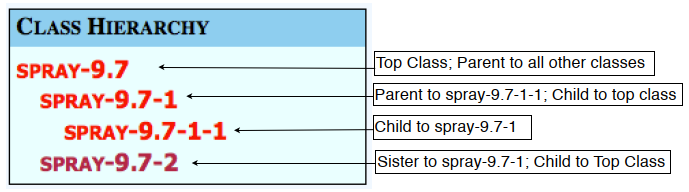
\includegraphics[width=11.03cm, height=2.76cm]{Class_hierarchy_for_spray-9_punk_7_class}
\caption{Class hierarchy for spray-9.7 class \cite{heck2014quality}}\label{fig:hierachy_class}
\end{figure}
Verb Classes are numbered according to shared semantics and syntax, and classes which share a top-level number (9-109) have corresponding semantic relationships. 

For instance, verb classes related to putting, such as put-9.1, put\_spatial-9.2, funnel-9.3, etc. are all assigned to the class number 9 and related to moving an entity to a location. 

Classes that share a top class can also be divided into subclasses, such as wipe verbs in wipe\_manner (10.4.1) and wipe\_inst (10.4.2) which specify the manner and instrument of wipe verbs in the \enquote{Verbs of Removing} group of classes (class number 10). 

An example of top-class numbers and their corresponding types is given in Table \ref{tb:vtype_example}. Class numbers 1-57 are drawn directly from Levin's (1993) classification. Class numbers 58-109 were developed later in the work of Korhonen \& Briscoe (2004). Notably, the verb types of the later classes are less general, as indicated by the fact that most of these classes have a one-to-one relationship between verb type and verb class.

\begin{figure}
\begingroup
\footnotesize
\centering
\begin{tabularx}{12cm}{l  l  l}
\hline
Class Number	&Verb Type	&Verb Class \\
\hline 
\hline
10&	Verbs of Removing		&banish-10.2 \\
&&cheat-10.6.1\\
&&clear-10.3\\
&&debone-10.8\\
&&fire-10.10\\
&&mine-10.9\\
&&pit-10.7\\
&&remove-10.1\\
&&resign-10.11\\
&&steal-10.5\\
&&wipe\_manner-10.4.1\\
\hline
26	&Verbs of Creation and Transformation	&adjust-26.9 \\
&&build-26.1 \\
&&convert-26.6.2\\
&&create-26.4\\
&&grow-26.2.1\\
&&knead-26.5\\
&&performance-26.7\\
&&rehearse-26.8\\
&&turn-26.6.1\\
\hline
13&	Verbs of Change of Possession	&berry-13.7 \\
&&contribute-13.2\\
&&equip-13.4.2\\
&&exchange-13.6.1\\
&&fulfilling-13.4.1\\
&&future\_having-13.3\\
&&get-13.5.1\\
&&give-13.1\\
&&hire-13.5.3\\
&&obtain-13.5.2\\
\hline
\end{tabularx}
\begin{TableCaption}
\caption{An example of top-class numbers and their corresponding verb-type\cite{verbnet_guidelines}}\label{tb:vtype_example}
\end{TableCaption}
\endgroup
\end{figure}
\subsection{Comparative Analysis} \label{sec_5_campare}
After a careful comparative analysis of WordNet, FrameNet, and VerbNet, we have determined that VerbNet is the most suitable lexical resource for our project. Its hierarchical categorization of verbs into classes provides a structured and comprehensive approach to understanding verb behavior, which is essential for our goal of generating transformation rules based on semantic interpretations of actions within user stories. 

VerbNet's organization aligns seamlessly with our project's requirements, offering the precision and granularity required for our semantic analysis and rule generation tasks.
Here are the three comparison key aspects:
\begin{itemize}
\item Focus: VerbNet is specialized in verbs, FrameNet offers broader coverage, including nouns and adjectives, and WordNet covers a wide range of words across different parts of speech.
\item Hierarchy: VerbNet and FrameNet provide hierarchical structures that help organize and understand word behavior, while WordNet focuses on synsets and relationships between words.
\item Applications: VerbNet is ideal for tasks related to verb semantics and actions. FrameNet is versatile for various lexical semantic tasks, and WordNet is widely used for word sense disambiguation and related applications.
\end{itemize}
\subsection{Bottom Line}\label{nlp_bottom_line}
For our Approach we identified VerbNet as the most appropriate lexical resource. Its methodical categorisation of verbs into hierarchical classes provides a structured and all-encompassing framework for understanding verb behavior. This alignment with our project goals is of utmost importance as it underpins our task of formulating transformation rules based on semantic interpretations of the actions (verbs) recognised by CRF and described in USs. VerbNet's organizational structure seamlessly matches the requirements of our project and ensures the necessary precision and granularity that are essential for our semantic analysis and rule generation.

